\documentclass[11pt,a4paper,openany,oneside]{book}

\usepackage[utf8]{inputenc}
\usepackage[english]{babel}
\usepackage{lmodern}
\usepackage{amsmath}
\usepackage{amsfonts}
\usepackage{amsthm}
\usepackage{hyperref}
\usepackage{booktabs}
\usepackage{array}
\usepackage{listings}
\usepackage{fixltx2e}
\usepackage{microtype}
\usepackage{textcomp}
\usepackage{color}
\usepackage{multirow}
\usepackage{graphicx}
\usepackage{fancyvrb}
\usepackage{dirtree}
\usepackage[Bjarne]{fncychap}

\newcommand{\vect}[1]{\mathbf{#1}}
\DeclareMathSymbol{\R}{\mathalpha}{AMSb}{"52}
\newcommand{\ra}[1]{\renewcommand{\arraystretch}{#1}}

\DefineVerbatimEnvironment{console}{Verbatim}{fontsize=\small}

\definecolor{listinggray}{gray}{0.9}
\definecolor{lbcolor}{rgb}{0.9,0.9,0.9}
\lstset{
	backgroundcolor=\color{lbcolor},
	tabsize=4,
	rulecolor=,
	language=matlab,
        basicstyle=\scriptsize,
        upquote=true,
        aboveskip={1\baselineskip},
        columns=fixed,
        showstringspaces=false,
        extendedchars=true,
        breaklines=true,
        prebreak = \raisebox{0ex}[0ex][0ex]{\ensuremath{\hookleftarrow}},
        frame=single,
        showtabs=false,
        showspaces=false,
        showstringspaces=false,
        identifierstyle=\ttfamily,
        keywordstyle=\color[rgb]{0.9,0,0.1},
        commentstyle=\color[rgb]{0.133,0.545,0.133},
        stringstyle=\color[rgb]{0.627,0.126,0.941},
}

\providecommand{\HUGE}{\Huge}% if not using memoir
\newlength{\drop}% for my convenience

\newcommand*{\titleGM}{\begingroup% Gentle Madness
\drop = 0.1\textheight
\vspace*{\baselineskip}
\vfill
\hbox{%
\hspace*{0.2\textwidth}%
\rule{1pt}{0.95\textheight}
\hspace*{0.05\textwidth}%
\parbox[b]{0.75\textwidth}{
\vbox{%
\vspace{\drop}
{\noindent\HUGE\bfseries \MakeUppercase{\toolboxname}\\[0.5\baselineskip]
User Manual}\\[2\baselineskip]
{\Large\itshape A MATLAB Toolbox for Fast Prototyping of \\ Machine Learning Simulations}\\[4\baselineskip]
{\Large SIMONE SCARDAPANE}\par
\vspace{0.4\textheight}
{
\noindent 
\includegraphics[scale=0.3]{./images/ispamm.png}}\\[\baselineskip]
}% end of vbox
}% end of parbox
}% end of hbox
\vfill
\null
\endgroup}

\newcommand{\toolboxname}{Lynx }

\begin{document}
\pagestyle{empty}
\titleGM
\clearpage

\tableofcontents

\frontmatter
\chapter*{Introduction}
\addcontentsline{toc}{chapter}{Introduction}

\section*{What is \toolboxname?}
\addcontentsline{toc}{section}{What is \toolboxname?}

Lynx is a research-oriented MATLAB toolbox for supervised and semi-supervised learning. It is aimed at making the comparison of multiple learning algorithms \textit{fast} to implement, \textit{simple} to modify, and easily \textit{repeatable} by others.

Its main idea is summarized in Fig. \ref{fig:generalschema}. Instead of writing yourself the code to organize the comparison, you can specify its details in a human-understandable configuration file, which is loaded by Lynx. At this point, the toolbox takes charge of everything else: importing the requested datasets, partitioning them, running the algorithms, collecting the results and analyzing them. Moreover, it can distribute such simulations on multiple threads, and multiple computers, using the Parallel Computing Toolbox\footnote{\url{http://www.mathworks.it/products/parallel-computing/}} and the Distributed Computing Server\footnote{\url{http://www.mathworks.it/products/distriben/}} of MATLAB.

\begin{figure}[t]
\centering
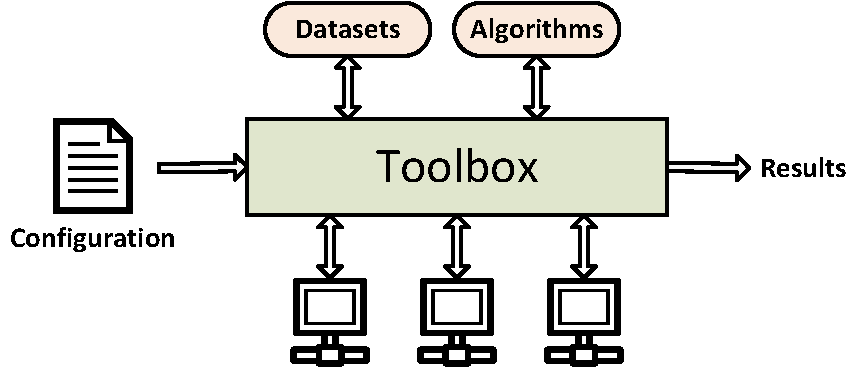
\includegraphics[scale=0.6]{./images/ToolboxSchema}
\caption{Schematic representation of the toolbox}
\label{fig:generalschema}
\end{figure}

In the configuration file, you can specify every detail of the simulation, including:

\begin{itemize}
\item the learning algorithms to use in the simulation,
\item which performance measures to compute (e.g. mean-squared error, ROC curves, etc.),
\item how to partition the data,
\item additional preprocessing steps for the datasets, or features for the algorithms (e.g. feature selection procedures),
\item enabling GPU support, saving the results, running a statistical test, and many other functionalities.
\end{itemize}

\section*{How do I read this manual?}

The strengths of Lynx, we hope, are more easily shown than said. Before starting, however, chapter \ref{chap:theoreticalbackground} summarizes briefly the essential concepts of supervised learning. Although most readers will be highly familiar with these, we use the chapter to introduce a small set of definitions around which the toolbox is organized, so we advise even the most experienced reader to a quick glimpse at the chapter.

Following this, chapter \ref{chap:install} details how to install the toolbox, and it contains a step-by-step guide to run two initial simulations. Then, chapter \ref{chap:writingconfig} and chapter \ref{chap:advancedfeatures} detail how to write your own configuration files, starting from the basic instructions (e.g. adding a dataset) up to the most advanced functionalities (e.g. parallelizing the experiments). Finally, it is time to develop your own classes: chapter \ref{chap:programminglynx} and chapter \ref{chap:advancedprogramming} present guided examples for implementing everything, including new learning algorithms, new performance measures, and even new learning tasks.

Additionally, we have included two appendices. Appendix \ref{chap:expfeatures} details experimental features we are working on, which have no support yet and that are expected to change rapidly over the course of the next months. Then, appendix \ref{chap:futuredevelopments} concludes by detailing some of other features we plan on implementing. We use this also to mention what we believe are the current ``weak'' points of the toolbox, that will require further development in the future.


\mainmatter
\chapter{First Use}
\label{chap:firstuse}
 
\section{Installing the Toolbox}
\label{sec:installation}

Once the toolbox has been download and extracted, it can be installed by running the file ``\textit{install.m}'' in the root folder. This adds all the toolbox folders to the search path of Matlab. Additionally, the installation script checks for the presence of any required external library. Currently, $3$ libraries are needed by the toolbox: LibSVM\footnote{\url{http://www.csie.ntu.edu.tw/~cjlin/libsvm/}}, the DeepLearn Toolbox\footnote{\url{https://github.com/rasmusbergpalm/DeepLearnToolbox}}, and the Kernel Methods Toolbox\footnote{\url{http://sourceforge.net/projects/kmbox/}}. None of them is essential, but some specific algorithms depend on them. If a library is not found, the installation script asks for the permission of downloading it and storing it in the ``lib'' folder:

\begin{console}
Checking for presence of Deep Learn Toolbox...
Deep Learn Toolbox not found. Do you want to install it? (Y/N) 
\end{console}

\noindent If the user denies the permission, the installation process continues, but the functionalities depending on the external library cannot be used. In this example, if the user denies the permission to install the DeepLearn Toolbox, a warning message will tell us that the \textit{StackedAutoEncoder} algorithm depends on it:
 
\begin{console}
Deep Learn Toolbox not found. Do you want to install it? (Y/N) N
You will not be able to use the StackedAutoEncoder algorithm
\end{console}
 
\noindent Due to the presence of a large set of folders, the search path is not saved by default. Hence, the installation script must be run every time Matlab is restarted. Alternatively, it is possible to save the path after the installation by running the built-in ``\textit{savepath}'' command. 

\section{Folder Structure}
\label{sec:folders}

Before continuing, let us look briefly at the folder structure of \toolboxname after the installation process. In Fig. \ref{fig:folders} we show a unix-like representation of the directories, together with a brief comment on their contents.

\begin{figure}[h]
\dirtree{%
.1 /.
.2 configs\DTcomment{Configuration files}. 
.2 core. 
.3 classes\DTcomment{Core classes of the toolbox}. 
.3 functions\DTcomment{Core functions of the toolbox}. 
.2 datasets\DTcomment{Available datasets}. 
.3 R. 
.3 BC. 
.3 (others). 
.2 functionalities\DTcomment{User-defined algorithms, etc.}. 
.3 algorithms. 
.3 performance. 
.3 preprocessors. 
.3 wrappers. 
.2 help\DTcomment{Help scripts for HTML reports}. 
.2 lib\DTcomment{External libraries}.
.2 manual\DTcomment{This manual folder}. 
.2 results\DTcomment{Saved results}. 
.2 scripts\DTcomment{Output scripts}. 
.2 tests\DTcomment{Testing suite}. 
.2 tmp\DTcomment{Temporary folder}. 
}
\label{fig:folders}
\caption{Folder Structure of the Toolbox}
\end{figure} 

\noindent Most of the directories contents are self-explanatory and will be explored in depth in the rest of this manual, but some general comments are in order. First, datasets are partitioned into multiple subfolders, corresponding to the internal concept of ``\textit{task}'', introduced in Section \ref{sec:understandingtasks}. All the user-defined functionalities, which can be roughly subdivided into $4$ families (learning algorithms, performance measures, preprocessors and wrappers) are stored in the corresponding subfolder of ``\textit{functionalities}''. Note that the toolbox already comes with several ready-to-use implementations and datasets. To get a general overview at the currently available functionalities and datasets, help scripts in the \textit{help} folder can be used to generate HTML reports. Internally, this is done using the Matlab Report Generator\footnote{\url{http://www.mathworks.it/products/ML_reportgenerator/}}. Output scripts are used for showing additional information after the simulation, and are introduced in Section \ref{sec:outputscripts}. The temporary folder is emptied at the end of every simulation, and whenever Matlab is closed. Finally, the toolbox is supplemented by a suite of unitary tests for checking the correctness of the code. This suite should be run every time a change is made to the code of the toolbox.

\section{General Workflow}

\begin{figure}
\centering
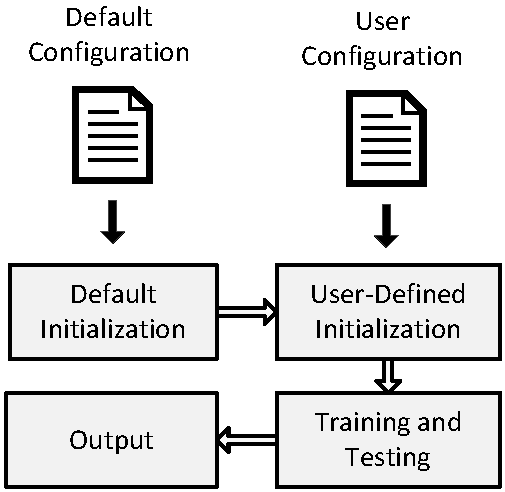
\includegraphics[scale=0.6]{./images/Workflow}
\caption{High-level Schema of the Execution of the Toolbox}
\label{fig:workflow}
\end{figure}

The general workflow of the toolbox is depicted in Fig. \ref{fig:workflow}. The simulation starts by loading a default configuration, saved in ``\textit{configs/default\_config.m}''. Then, the user-defined configuration is loaded, corresponding to the file ``\textit{config.m}'' in the root folder of the toolbox. In this file, the user can specify what algorithms must be tested, and on which datasets. Additionally, it is possible to override some general behavior of the toolbox, and to enable some advanced features, such as parallelization of the experiments.

According to these requirements, the toolbox trains and tests a set of models on the requested data, and at the end shows on the console the average training times and testing accuracies. To understand briefly the training phase, consider the simplest case of a single algorithm, tested on a single dataset, using a random partition of the data. The worflow of execution is detailed in Fig. \ref{fig:trainingphase}. The dataset is loaded from memory and preprocessed using a set of methods specified in the configuration file. Then, the preprocessed dataset is subdivided into a training set and a testing set. The training set is then passed in input to a learning algorithm, to build a suitable model. The learning algorithm can be encapsulated into one (or more) wrappers, allowing for the possibility of fine-tuning its parameters, choosing the right subset of input features, and many additional functionalities. Finally, the testing set is passed as input to the model, which provides a set of predicted outputs. This outputs are compared with the expected ones using a given measure of accuracy, that determines the final testing error of the algorithm. All the blocks of Fig. \ref{fig:trainingphase} are fully configurable and extensible.

\begin{figure}
\centering
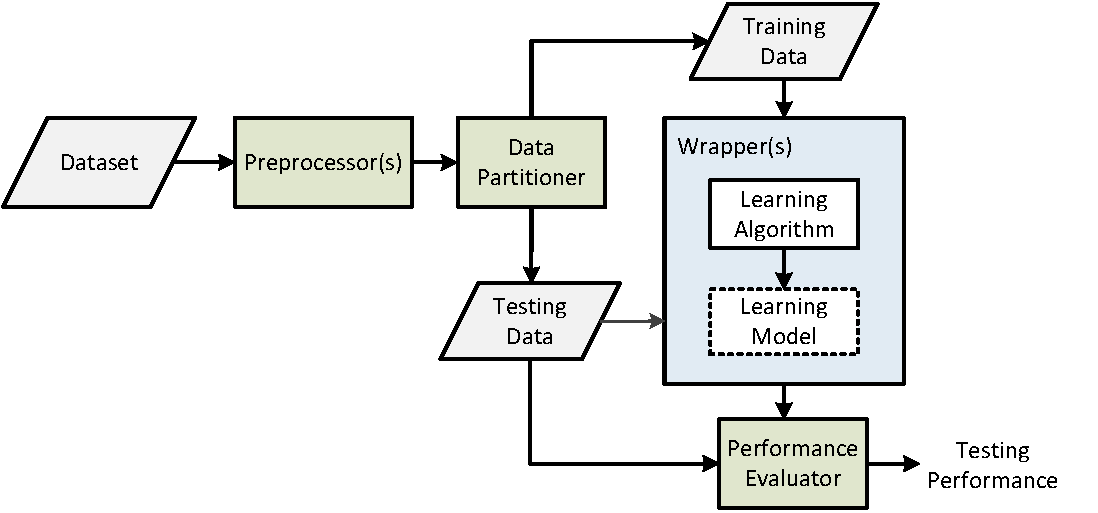
\includegraphics[scale=0.75]{./images/Disegno3}
\caption{Schematic Depiction of the Training Phase}
\label{fig:trainingphase}
\end{figure}

In the more general case, the data can be split according to a $k$-fold cross validation, hence the training/testing process is repeated $k$ times and results are averaged. This can be repeated for multiple algorithms and datasets, although the preprocessing step and the partitioning steps are common to all the algorithms so as to ensure a fair comparison. Additionally, the overall process can be repeated multiple times (\textit{runs}).

\section{Running the First Test}
\label{sec:runningfirsttest}
To help familiarizing with the software, the configuration file already contains the instructions to run a very simple experiment. 
Although its syntax is explored in detail in the following chapter, for the sake of this demo it is enough to understand that this example requires the test of two different learning algorithms:

\begin{lstlisting}
add_algorithm('B', 'Baseline', @Baseline);
add_algorithm('ELM', 'Extreme Learning Machine', @ExtremeLearningMachine);
\end{lstlisting}

\noindent The ``baseline'' algorithm is a dummy learning algorithm who, in this case, always outputs the mean value of its training set. The second algorithm is a more sophisticated Extreme Learning Machine trained using an $L2$-regularized ridge regression \cite{Huang2012}. The test is executed on a single dataset taken from the UCI repository\footnote{\url{http://archive.ics.uci.edu/ml/}}:

\newpage

\begin{lstlisting}[language=matlab]
add_dataset('G', 'Glass', 'uci_glass');
\end{lstlisting}

\noindent In this case, we have no wrappers and no preprocessors. The simulation is started by executing the ``\textit{run\_simulation.m}'' script in the root folder. The result of the simulation is then printed on the console. Below we provide a small description of each phase.

\subsection{Initialization Phase}

In the initialization phase, the configuration file is read and all the data structures are initialized:

\begin{console}
Initializing simulation...
Current seed for prng: 1340863332
End of initialization, will test 2 algorithm(s) on 1
   dataset(s) for 1 time(s)
\end{console}

\noindent Other preliminary actions are eventually run in this phase. For example, the toolbox checks the compatibility of all the algorithms with the requested datasets (see next section); it activates a pool of threads if parallelization is requested; and so on.

\subsection{Training Phase}

In the training phase, each algorithm is run on every dataset in turn. In this case, the default configuration specifies to execute a $3$-fold cross validation, and a single run:

\begin{console}
Testing Extreme Learning Machine on Glass (run 1/1)
   Fold 1... 
   Fold 2... 
   Fold 3... 
Testing Baseline on Glass (run 1/1)
   Fold 1... 
   Fold 2... 
   Fold 3... 
\end{console}

\subsection{Output Phase}
\label{sec:outputphase}

In the output phase, the results, in the form of mean and standard deviation of the errors and the training times, are printed on screen. As an example, these are typical average errors for the demo:

\begin{console}
Average error:
       Baseline  Extreme Learning Machine
Glass     1.014                    0.5375
\end{console}

Note that the actual meaning of the numbers may vary depending on the dataset. This is explained in more detail in the next section.

After this step, an optional statistical testing is executed. See Section \ref{sec:statistical_testing} for information on how to request it. Currently supported statistical tests include a Wilcoxon signed rank test \cite{dietterich1998approximate}, and a Friedman test \cite{demvsar2006statistical}. Additional output scripts can be added to the simulation for gathering information on the run. This functionality is explored in Section \ref{sec:outputscripts}.

\section{Understanding Tasks and Analyzing the Output}
\label{sec:understandingtasks}

\vspace{-2em}

\begin{center}
\begin{table}
{\centering\hfill{}
\begin{tabular}{lll}
\toprule
ID & Input & Output \\ 
\midrule
R (Regression) & \multirow{3}{*}{$\vect{X} \in \R^{N \times d}$ } & $\vect{y} \in \R^N$ \\
BC (Binary Classification) & & $\vect{y} \in \left\{-1,+1\right\}^N$\\
MC (Multiclass Classification) & & $\vect{y} \in \left\{1,\dots,M\right\}^N$\\
\bottomrule
\end{tabular}}
\hfill{}
\caption{Summary of the basic tasks defined in the toolbox}
\label{tab:basictasks}
\end{table}
\end{center}

\subsection{Basic Tasks}

To understand the results, a few more details on the structure of the toolbox is required. Speaking broadly, a dataset is composed of an $N \times d$ matrix of real values (currently, categorical variables are not supported), and a $N \times 1$ vector of targets, where $N$ is the number of examples available to the system, and $d$ is the input dimensionality. That is, each row in the input matrix is an observation, whereas each column is a feature.

A \textit{task} identifies the type of learning problem of a given dataset, which changes the type of the requested output. The following basic tasks are currently defined:

\begin{description}
\item[Regression (R)]: the output is a single real number.
\item[Binary Classification (BC)]: the output is an integer number in the set $\left\{-1,+1\right\}$.
\item[Multiclass Classification (MC)]: the output is an integer number in the set $\left\{1,\dots,M\right\}$, where $M$ is the number of classes.
\end{description} 
	
These are summarized in Table \ref{tab:basictasks}. An algorithm can be defined to work on one or more of them. For example, a particular algorithm can be defined only for classification tasks, i.e. BC and MC tasks, but not for regression tasks. If in the simulation some inconsistencies are found (i.e., an algorithm is tested on an unsupported task), they are listed in the beginning and the statistical testing is avoided. The following is an example of the corresponding warning message:

\begin{console}
The following tests are not possible:
	 KRLS on Yeast.
Statistical testing will not be executed.
\end{console}

\noindent Successively, the corresponding training phase is skipped:

\begin{console}
Testing KRLS on Yeast (run 1/1)
	Not Allowed
\end{console}

\subsection{Complex Tasks}

\vspace{-2em}

\begin{center}
\begin{table}[t]
{\centering\hfill{}
\begin{tabular}{llll}
\toprule
ID & Input & Output \\ 
\midrule
PR (Prediction) & $\vect{x} \in \R^N$ & NA \\
ML (Multilabel Classification) & $\vect{X} \in \R^{N \times d}$ & $\left\{ \vect{y}_i \right\}, \vect{y}_i = \left\{-1, +1\right\}^N$ \\
\bottomrule
\end{tabular}}
\hfill{}
\caption{Summary of the complex tasks defined in the toolbox}
\label{tab:complextasks}
\end{table}
\end{center}

Clearly, the tasks of Table \ref{tab:basictasks} do not cover all the possibilities arising in supervised learning. For this reason, the toolbox identifies a set of non-basic tasks, i.e., tasks that do not conform to the previous description. Practically, what changes is either the semantic of the problem, or the way in which the data is stored on the disk. A non-basic task is handled by previously transforming it into one or more basic tasks. Currently, two non-basic tasks are defined: 

\begin{description}
\item[Prediction (PR)]: here the input is a vector containing the ordered samples of a time-invariant time series, and the required output is a one-step ahead prediction. This is handled by transforming it into a regression problem, where the input is an embedding of the previous $r$ values of the time-series, with $r$ specified by the user. If the time series has $N$ values, $N-r$ examples are constructed.

\item[Multilabel (ML)]: this is the case where a given number $T$ of binary classification problems are defined on the same input matrix. This is handled by constructing $T$ separate binary classification tasks during the initialization phase.
\end{description}

The structure of each complex task is summarized in Table \ref{tab:complextasks}. In Table \ref{tab:correspondeces}, instead, we show how each complex task is handled by the toolbox.

\begin{center}
\begin{table}[t]
{\centering\hfill{}
\begin{tabular}{ll}
\toprule
Original Task & Transformed Tasks \\ 
\midrule
PR & A single R task.  \\
ML & Multiple BC tasks. \\
\bottomrule
\end{tabular}}
\hfill{}
\caption{Transformations between Complex Tasks and Basic Tasks}
\label{tab:correspondeces}
\end{table}
\end{center}

\subsection{Training Performance}

The measure of performance shown in the results changes depending on the task associated to each dataset. By default, the misclassification rate is shown for classification tasks, while the Normalized Root Mean-Squared error \footnote{\url{http://en.wikipedia.org/wiki/Root-mean-square_deviation}} for regression, defined as:

\begin{equation}
\text{NRMSE}(\vect{y}, \vect{d}) = \sqrt{\frac{\sum_{i=1}^N (d_i-y_i)^2}{N \hat{\sigma}_y}}
\label{eq:nrmse}
\end{equation}

\noindent where $\vect{y}$ are the expected outputs, $\vect{d}$ are the actual outputs, $N$ is the cardinality of both $\vect{y}$ and $\vect{d}$, and $ \hat{\sigma}_y$ is an empirical estimate of the variance of $\vect{y}$. The measure of error is averaged over all the folds and all the runs.

As an example, consider the sample run of Section \ref{sec:outputphase}. Since the Glass dataset is a regression task, the numbers that appear in the console are the NRMSE computed over the testing set, averaged over the different folds. The default performance measures can be changed by the user, a functionality explored in Section \ref{sec:changingperformance}. Also, new performance measures can be defined, see Section \ref{sec:implementingperformancemeasures}. 

\chapter{Writing a Configuration File}
\label{chap:configfile}

\section{General Configuration}
\label{sec:generalconfig}

Referring again to Fig. \ref{fig:workflow}, remember that the default parameters governing the behavior of the simulation are stored in the file ``\textit{configs/default\_config.m}''. This file is loaded automatically by the toolbox before loading the user-defined one. Hence, each setting defined in the default configuration can be adapted by simply redefining it in the user-defined configuration file, which effectively overwrites the default parameter.

Below is a list of the most important parameters defined in the default config file:

\begin{itemize}
\item \verb;nRuns; : the number of times the simulation will be run. As an example, if \verb;nRuns; is set equal to $2$, each test will be performed twice. This defaults to $1$.
\item \verb|partition_strategy|: an object describing how the toolbox should subdivide the data for testing. This can be any object of class \verb|PartitionStrategy|. Currently, two possibilities are available:

\begin{itemize}
\item \verb|partition_strategy| can be an object of class \verb|HoldoutPartition|, in which case a specified fraction of data will be kept for testing (this is called \textit{holdout}). For example, by setting:

\begin{lstlisting}
partition_strategy = HoldoutPartition(0.3);
\end{lstlisting}

each algorithm will be trained on a randomly selected $70\%$ of the data, and tested on the remaining $30\%$.

\item \verb|partition_strategy| can be an object of class \verb|KFoldPartition|, in which case a $k$-fold cross validation is performed. Typical values of folds in this case are between $3$ and $10$.

\end{itemize}


The default behavior is a $3$-fold cross-validation. Note that the partitioning strategy can equivalently be set using the \verb|set_partition_strategy| method.

\item \verb|seed_prng|: the seed for initializing the pseudo-random number  of Matlab. This can be an integer number or the string ``shuffle'' (default value), in which case a random seed is used. In the latter case, the random seed is printed on screen for allowing the repetition of the exact experiment.
\end{itemize}

\noindent Hence, the default configuration comprises the following parameters:

\begin{lstlisting}
nRuns = 1;
partition_strategy = KFoldPartition(3);
seed_prng = 'shuffle';
\end{lstlisting}

\noindent Note that configuration files can be easily nested. As an example, suppose we have a range of configurations (e.g. a set of algorithms or datasets) that we include frequently in our simulations. These can be written on a particular file, e.g. ``\textit{configs/own\_config.m}'', and imported when needed in the standard configuration file:

\begin{lstlisting}
own_config.m;
\end{lstlisting}


\section{Adding an Algorithm}

An algorithm can be added to the simulation with the following syntax:

\begin{console}
add_algorithm(ID, name, pointer, varargin);
\end{console}

\noindent where:

\begin{itemize}
	\item \verb|ID| is a unique string for identifying the algorithm in the simulation,
	\item \verb|name| is the algorithm’s name (to be displayed in the results),
	\item \verb|pointer| is a pointer to the algorithm’s class,
	\item \verb|varargin| are the additional parameters to be passed to the constructor.
\end{itemize}

\noindent As in the standard convention of Matlab coding, additional parameters are composed as follows:

\begin{itemize}
	\item One or more required parameters,
	\item One or more additional parameters,
	\item One or more name/value pairs. As a general rule, most parameters are in this form.
\end{itemize}

\noindent For example, the following call:

\begin{lstlisting}
add_algorithm('NN', 'Neural Net', @MultilayerPerceptron);
\end{lstlisting}

\noindent adds a default-initialized Multilayer Perceptron to the simulation. Similarly, the call:

\begin{lstlisting}
add_algorithm('NN', 'Neural Net', @MultilayerPerceptron, 'hiddenNodes', 15);
\end{lstlisting}

\noindent adds a Multilayer Perceptron, with $15$ nodes in the hidden layer.

A concise HTML report with a list of all implemented algorithms and respective parameters can be found by calling the script ``\textit{help/info\_algorithms.m}''. Additional information on each algorithm can be found by visualizing the help for the respective class.

\section{Adding a Wrapper}

A wrapper provides additional functionalities to an algorithm (called in this context its \textit{base algorithm}) by encapsulating its behavior and intercepting inputs and outputs to its training and testing functions. Wrappers can be used for fine-tuning model parameters, extracting or selecting features, saving the models resulting from the simulation, etc.

The syntax for adding a wrapper is similar to the syntax for adding an algorithm:

\begin{console}
add_wrapper(ID, wrapper, varargin);
\end{console}

\noindent Where:

\begin{itemize}
\item \verb|ID| is the ID of the algorithm to be encapsulated,
\item \verb|wrapper| is a pointer to the wrapper’s class,
\item \verb|varargin| are the additional parameters for the wrapper.
\end{itemize}

\noindent Consider as an example the following call:
\begin{lstlisting}
add_wrapper('NN', @Featuresearch_GA);
\end{lstlisting}

\noindent This adds a wrapper to the Multilayer Perceptron defined in the previous section, that runs a genetic algorithm for searching the optimal subset of features. For details on the implemented wrappers and required parameters, the script ``\textit{help/info\_wrappers.m}'' generates a concise report. More information on each wrapper is available by visualizing the help for the corresponding class.

It is important to note that wrappers can pile on top of each other:

\begin{console}
add_wrapper(ID, wrapper1, ...);
add_wrapper(ID, wrapper2, ...);
\end{console}

In this case, the \textit{wrapper2} is executed by using as a base algorithm the \textit{wrapper1}, which in turn uses as a base class the algorithm identified by ID. Consider the following:

\begin{lstlisting}
add_wrapper('NN', @Featuresearch_GA);
add_wrapper('NN', @OneVersusAll);
\end{lstlisting}

\noindent In this case, for a multiclass classification problems with $M$ classes $M$ different neural networks are trained. Each network will have a different subset of input parameters, found by the genetic search. The order in which the wrappers are stacked is very important. The following call is different from the previous one:

\begin{lstlisting}
add_wrapper('NN', @OneVersusAll);
add_wrapper('NN', @Featuresearch_GA);
\end{lstlisting}

\noindent Here, a single genetic search is executed, and internally the algorithm is trained using a one-versus-all strategy.

Many wrappers require a parameter designating how to subdivide the data for performing a validation step. In this case, this parameter follows the same semantic as the \verb|testParameter| defined for the general configuration.

\subsection{Performing a Parameter Sweep}
\label{sec:parametersweep}

A very common need in supervised learning is testing a given set of values of one or more parameters of an algorithm, then choosing the combination resulting in the highest level of accuracy. In the toolbox, this functionality is provided natively by the \textit{ParameterSweep} wrapper. As an example of its usage, consider the Extreme Learning Machine (ELM) adopted in the sample configuration, whose simulation has been analyzed in the previous chapter. It has two parameters, a regularization factor (denoted by \verb|regularizationFactor|) and a kernel parameter (denoted by \verb|kernel_para|). As is standard practice, we want to test the following range of values for each parameter:

\begin{equation}
2^{-5}, 2^{-4}, \dots, 2^{5}
\end{equation}

\noindent Since we have two parameters, this results in $10 \times 10 = 100$ configurations to be tested. The validation accuracy of each configuration should be computed by performing an inner $3$-fold cross validation on the training data. The following command generates the corresponding wrapper in our example:

\newpage

\begin{lstlisting}
add_wrapper('ELM', @ParameterSweep, 3, {'regularizationFactor', 'kernel_para'}, {'exp', 'exp'}, [-5 5; -5 5], [1 1]);
\end{lstlisting}

\noindent Although this may seem daunting at first, it is actually rather simple. The first parameter has a semantic similar to the \verb|testParameter| discussed in Section \ref{sec:generalconfig}, and it instructs the wrapper to perform a $3$-fold cross validation. This is followed by a cell array with the names of the parameters to be tested. The next cell array tells the wrapper that the values must be computed in an exponential fashion, i.e., by powers of $2$. Then, we provide the lower and upper bounds for each parameter, and the step values for computing the ranges.

\subsection{Saving and Loading a Configuration}

The second common requirement that we analyze here briefly is that of saving the configuration of an algorithm, for retrieving it in a following simulation. As an example, the grid search of the previous subsection requires training and testing $100$ models, each time performing a $3$-fold cross validation. For large datasets, this requires a very large time, hence we would like to save the results for loading it successively. The \textit{SaveConfiguration} wrapper can be used for saving a configuration:

\begin{lstlisting}
add_wrapper('ELM', @SaveConfiguration, 'ELM_SAVED', './sweeps');
\end{lstlisting}

\noindent After training a model, this will be saved in the ``\textit{./sweeps}'' folder. Note that a simulation requires training several models, one for each fold and dataset. Hence, this will save several files in the folder. The naming convention is that a file is denoted as ID\_DATASET\_FOLD.mat, where ID is the id defined above (ELM\_SAVED in our example), DATASET is the name of the dataset, and FOLD is the numerical id of the fold. The saved models can be retrieved on a successive simulation using the \textit{LoadConfiguration} wrapper:

\begin{lstlisting}
add_wrapper('ELM', @LoadConfiguration, './sweeps', 'ELM_SAVED', {'regularizationFactor', 'kernel_para'});
\end{lstlisting}

\noindent Note that this wrapper requires explicitly a list of training parameters to be loaded.

\section{Adding a Dataset}

A new dataset can be added to the simulation with the following syntax:

\begin{console}
add_dataset(ID, name, dataset, [subsample], varargin);
\end{console}

Where:

\begin{itemize}
\item \verb|ID| is a string identifying the dataset in the simulation,
\item \verb|name| is a name for the dataset, to be displayed in the results,
\item \verb|dataset| is the unique alphanumerical string denoting the dataset in the filesystem,
\item \verb|subsample| is a percentage of the dataset to load (optional),
\item \verb|varargin| are additional parameters to be given in specific cases.
\end{itemize}

\noindent As an example, the call:

\begin{lstlisting}
add_dataset('Y', 'Yacht', 'uci_yacht');
\end{lstlisting}

\noindent adds the dataset ``\textit{uci\_yacht}'' to the simulation with name ``Yacht'', while:

\begin{lstlisting}
add_dataset('Y', 'Yacht', 'uci_yacht', 0.5);
\end{lstlisting}

\noindent adds the same dataset, but loads only a randomly chosen 50\% of it. A list of available datasets (and respective ids) can be obtained by calling ``\textit{help/info\_datasets.m}''. The datasets are divided depending on the task. Below we provide more information on the way in which each complex task can be loaded.

\subsection{Adding a Prediction Dataset}

In the case of a prediction task, the toolbox requires the embedding dimension for the input vector:

\begin{lstlisting}
add_dataset('MG', 'Mackey-Glass', 'mackeyglass', 1, 'embeddingFactor', 7);
\end{lstlisting}

\noindent Note that in this case it is necessary to specify a subsampling percentage.

\subsection{Adding a Multi-label Dataset}
\label{sec:chap2:multilabeldataset}

Remember from Section \ref{sec:understandingtasks} that a multi-label task with $M$ labels is loaded as $M$ different binary classification tasks. The name of each of these sub-tasks is created from the name provided by the user and an additional string contained in the dataset. The id, instead, is created sequentially starting from the user-defined id. As an example, suppose \textit{ml\_example} is a multi-label dataset consisting of $3$ labels. Consider the following call:

\begin{lstlisting}
add_dataset('EX', 'Multi-Label Dataset', 'ml_example');
\end{lstlisting}

\noindent This call creates $3$ distinct binary classification tasks, with ids given by EX-1, EX-2, and EX-3.

\section{Adding a Preprocessor to a Dataset}

A preprocessor applies some specific transformation to a dataset in the initialization phase. A preprocessor can be added with the following syntax:

\begin{console}
add_preprocessor(ID, preprocessor, varargin);
\end{console}

\noindent Where:

\begin{itemize}
\item \verb|ID| is a regular expression that should match with all the datasets ids to which the preprocessor should be applied,
\item \verb|preprocessor| is a pointer to the preprocessor’s class,
\item \verb|varargin| are the additional parameters of the preprocessor.
\end{itemize}

\noindent As an example, the call:

\begin{lstlisting}
add_preprocessor('Y', @ApplyPca, 'varianceToPreserve', 0.95);
\end{lstlisting}

\noindent applies a PCA transformation to the dataset previously defined, retaining only the principal components encompassing at least 95\% of the variance of the original input.

A list of the available preprocessors is obtained by calling the script ``\textit{help/info\_preprocessors.m}''. Additional information on each preprocessor is given by the help of the corresponding class.

\subsection{Preprocessors and Multi-label Tasks}

The fact that the syntax for adding a pre-processor accepts a regular expressions is particularly suited for multi-label tasks. Continuing the example of Section \ref{sec:chap2:multilabeldataset}, suppose we now want to perform a PCA on all three binary classification tasks. This can be done with a single call:

\begin{lstlisting}
add_preprocessor('EX-.', @ApplyPca, 'varianceToPreserve', 0.95);
\end{lstlisting}

\noindent The regular expression follows the standard Matlab convention: in particular, the dot refers to ``any character'', allowing to match all three datasets together. More information on the syntax of regular expressions can be found by reading the help of the built-in ``\textit{regexp}'' function.

\section{Choosing a Statistical Test}

A statistical testing is requested by calling the following method:

\begin{lstlisting}
set_statistical_test(class);
\end{lstlisting}

\noindent where \verb|class| is a pointer to a class deriving from \verb|StatisticalTest|. Each statistical test has certain conditions that must be satisfied so that it can be called. As an example, the Wilcoxon signed-rank text requires exactly two algorithms and at least two datasets. So, if we add it to a simulation like:

\begin{lstlisting}
set_statistical_test(@WilcoxonTest);
\end{lstlisting}

\noindent but we do not respect the conditions, a critical error is issued during the initialization phase.
\chapter{Writing a configuration file}
\label{chap:writingconfig}

In this chapter, you will learn the basics for writing a configuration file. We focus on the essential elements, i.e. adding models, datasets, wrappers and preprocessors. For additional features, refer to the next chapter.

\section{Adding a dataset}

Datasets are stored in the ``\textit{datasets}'' folder of the toolbox. They are organized in folders corresponding to the different tasks. To get a summary of available tasks and datasets, run the \verb|info_datasets.m| script.

A new dataset can be added to the simulation with the following syntax:

\begin{small}
\begin{verbatim}
add_dataset(id, name, filename);
\end{verbatim}
\end{small}

\noindent where:

\begin{itemize}
\item \verb|id| is a string identifying the dataset in the configuration file,
\item \verb|name| is a name for the dataset, to be displayed in the results,
\item \verb|filename| is the unique alphanumerical string denoting the dataset in the filesystem.
\end{itemize}

\noindent As an example, the call:

\begin{lstlisting}
add_dataset('Y', 'Yacht', 'uci_yacht');
\end{lstlisting}

\noindent adds the dataset ``\textit{uci\_yacht}'' to the simulation with name ``Yacht''.

\subsection{Adding a multilabel dataset}
\label{sec:multilabeldataset}

You may have seen during the simulation that the multilabel classification task has no performance measure assigned to it. This is because it is an ``\textit{incomplete}'' data type, i.e., a data type for which no training algorithms is available. A similar thing can be said about time-series inputs, which cannot currently be used directly by any model. Hence, they are handled by transforming them (after loading the datasets) into other, more ``basic'' tasks. In particular:

\begin{itemize}
\item Time-series datasets are transformed into regression datasets by embedding the time-series into a phase space.
\item Multilabel classification tasks are transfomed into multiple binary classification tasks (the so-called \textit{binary relevance} method).
\end{itemize}

As an example, try to add a multilabel dataset to a simulation:

\begin{lstlisting}
add_dataset('C', 'Cal 500', 'cal500_mood);
\end{lstlisting}

\noindent You can see that, during initialization, the $36$ labels in the dataset are transformed into $36$ different binary classification datasets:

\begin{console}
Extracted 36 different binary classification datasets from original
  dataset Cal 500
\end{console}

\noindent The $36$ tasks have sequential ids given by C-1, C-2, etc. Similarly, try to add a dataset with a time-series as input:

\begin{lstlisting}
add_dataset('M', 'Mackey-glass', 'mackeyglass');
\end{lstlisting}

\noindent During initialization, this is transformed into a regression dataset:

\begin{console}
Embedded dataset Mackey-glass, 4993 samples extracted
\end{console}

How to ``complete'' these tasks, and how to design new ones, are topics explored in the last chapter of the manual.

\section{Adding a model}

A model can be added to the simulation with the following syntax:

\begin{lstlisting}
add_model(id, name, pointer, varargin);
\end{lstlisting}

\noindent where:

\begin{itemize}
	\item \verb|id| is a unique string for identifying the algorithm in the simulation,
	\item \verb|name| is the algorithm's name (to be displayed in the results),
	\item \verb|pointer| is a pointer to the algorithm's class,
	\item \verb|varargin| are the additional parameters to be passed to the constructor of the model.
\end{itemize}

\noindent As in the standard convention of Matlab coding, additional parameters are composed as follows:

\begin{itemize}
	\item One or more required parameters,
	\item One or more additional parameters,
	\item One or more name/value pairs. As a general rule, most parameters are in this form.
\end{itemize}

\noindent For example, the following call:

\begin{lstlisting}
add_model('SVM', 'Support Vector Machine', @SupportVectorMachine);
\end{lstlisting}

\noindent adds a default-initialized Support Vector Machine to the simulation. Similarly, the call:

\begin{lstlisting}
add_model('SVM', 'Support Vector Machine', @SupportVectorMachine, 'kernel_type', 'lin');
\end{lstlisting}

\noindent adds a Support Vector Machine with a linear kernel.

A concise HTML report with a list of all implemented models and respective parameters can be found by calling the script \verb|info_models.m|. Additional information on each model can be found by visualizing the help for the respective class.

\subsection{Changing the training algorithm}

Each model has a default training algorithm, that can be changed with the \verb|set_training_algorithm| function. For example, to change the training algorithm of the previously defined Support Vector Machine to LibSVM:

\begin{lstlisting}
set_training_algorithm('SVM', @LibSVM); 
\end{lstlisting}

\noindent Available training algorithms are listed in the \verb|info_models.m| script.

\section{Adding a preprocessor}

A preprocessor applies some specific transformation to a dataset in the initialization phase. A preprocessor can be added with the following syntax:

\begin{lstlisting}
add_preprocessor(id, preprocessor, varargin);
\end{lstlisting}

\noindent Where:

\begin{itemize}
\item \verb|id| is a regular expression that should match with all the datasets ids to which the preprocessor should be applied,
\item \verb|preprocessor| is a pointer to the preprocessor's class,
\item \verb|varargin| are the additional parameters of the preprocessor.
\end{itemize}

\noindent As an example, the call:

\begin{lstlisting}
add_preprocessor('Y', @PrincipalComponentAnalysis, 'varianceToPreserve', 0.95);
\end{lstlisting}

\noindent applies a PCA transformation to the dataset previously defined, retaining only the principal components encompassing at least 95\% of the variance of the original input.

A list of the available preprocessors is obtained by calling the script \verb|info_preprocessors.m|. Additional information on each preprocessor is given by the help of the corresponding class.

\subsection{Preprocessors and Multi-label Tasks}

The fact that the syntax for adding a preprocessor accepts a regular expression is particularly suited for multi-label tasks. Continuing the example of Section \ref{sec:multilabeldataset}, suppose we now want to perform a PCA on all $36$ binary classification tasks. This can be done with a single call:

\begin{lstlisting}
add_preprocessor('C-.', @PrincipalComponentAnalysis, 'varianceToPreserve', 0.95);
\end{lstlisting}

\noindent The regular expression follows the standard MATLAB convention: in particular, the dot refers to ``any character'', allowing to match all three datasets together. More information on the syntax of regular expressions can be found by reading the help of the built-in \verb|regexp| function.

\section{Adding a wrapper}

A wrapper provides additional functionalities to an algorithm (called in this context its \textit{base algorithm}) by encapsulating its behavior and intercepting inputs and outputs to its training and testing functions. Wrappers can be used for fine-tuning model parameters, extracting or selecting features, saving the models resulting from the simulation, etc.

The syntax for adding a wrapper is similar to the syntax for adding an algorithm:

\begin{lstlisting}
add_wrapper(id, wrapper, varargin);
\end{lstlisting}

\noindent Where:

\begin{itemize}
\item \verb|id| is the ID of the algorithm to be encapsulated,
\item \verb|wrapper| is a pointer to the wrapper’s class,
\item \verb|varargin| are the additional parameters for the wrapper.
\end{itemize}

\noindent Consider as an example the following call:
\begin{lstlisting}
add_wrapper('SVM', @Featuresearch_GA);
\end{lstlisting}

\noindent This adds a wrapper to the Multilayer Perceptron defined in the previous section, that runs a genetic algorithm for searching the optimal subset of features. For details on the implemented wrappers and required parameters, the script \verb|info_wrappers.m| generates a concise report. More information on each wrapper is available by visualizing the help for the corresponding class.

It is important to note that wrappers can pile on top of each other:

\begin{lstlisting}
add_wrapper(ID, wrapper1, ...);
add_wrapper(ID, wrapper2, ...);
\end{lstlisting}

In this case, the \textit{wrapper2} is executed by using as a base algorithm the \textit{wrapper1}, which in turn uses as a base class the algorithm identified by ID. As an example, consider the following code:

\begin{lstlisting}
add_wrapper('SVM', @Featuresearch_GA);
add_wrapper('SVM', @SaveConfiguration);
\end{lstlisting}

\noindent In this case, the first wrapper searches for the optimal feature subset using a genetic algorithm, while the second wrapper saves the resulting configuration, as shown in Fig. \ref{fig:wrappersexample}.

\begin{figure}[t]
\centering
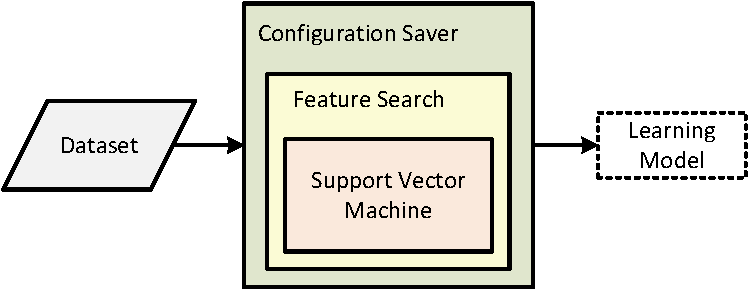
\includegraphics[scale=0.6]{./images/WrappersExample}
\caption{Example of piling two different wrappers}
\label{fig:wrappersexample}
\end{figure}

\noindent The wrappers act at different moments during the learning process: the first one searches the subset before training the final SVM, while the second wrapper saves the configuration after the final training. Other wrappers can have different effects also in the testing phase, allowing for the creation of complex behaviors. For example, an unfolded version of Fig. \ref{fig:wrappersexample} is shown in Fig. \ref{fig:wrappersexample_unfolded}.

\begin{figure}[t]
\centering
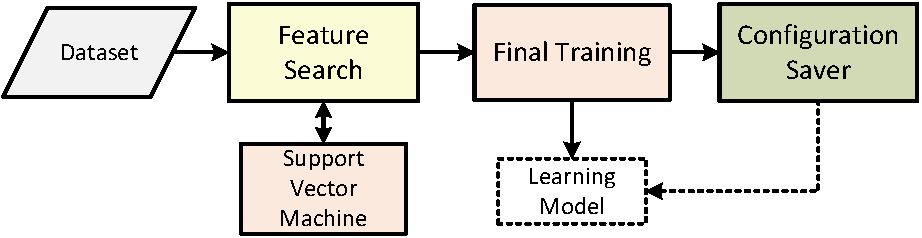
\includegraphics[scale=0.6]{./images/WrappersExampleUnfolded}
\caption{Same as Fig. \ref{fig:wrappersexample}, but with the actions of the wrappers unfolded in time.}
\label{fig:wrappersexample_unfolded}
\end{figure}

\subsection{Example 1: Performing a parameter sweep}
\label{sec:parametersweep}

A very common need in supervised learning is testing a given set of values of one or more parameters of an algorithm, then choosing the combination resulting in the highest level of accuracy. In the toolbox, this functionality is provided natively by the \verb|ParameterSweep| wrapper. As an example of its usage, consider the Extreme Learning Machine (ELM) adopted in the sample configuration, whose simulation has been analyzed in the previous chapter. It has (between others) two tunable parameters, a regularization factor (denoted by \verb|regularizationFactor|) and the number of hidden nodes (denoted by \verb|hiddenNodes|). As is standard practice, we want to test the following range of values for the parameters:

\begin{eqnarray}
2^{-5}, 2^{-4}, \dots, 2^{5} \text{ for the regularization factor}\\
100, \dots, 1000 \text{ for the number of hidden nodes}
\end{eqnarray}

\noindent Since we have two parameters, this results in $10 \times 9 = 90$ configurations to be tested. The following command generates the corresponding wrapper in our example:

\begin{lstlisting}
add_wrapper('ELM', @ParameterSweep, {'regularizationFactor', 'hiddenNodes'}, {2.^-5:5, 100:100:1000});
\end{lstlisting}

\noindent Although this may seem daunting at first, it is actually rather simple. The first parameter is a cell array with the names of the parameters to be tested. The second parameter is a cell array with the values to be tested. By default, this wrapper uses a $3$-fold cross-validation on the training data to test the accuracy. We may change this with any object of class \verb|PartitionStrategy|. For example, to execute an holdout partitioning with $30\%$ of validation data:

\begin{lstlisting}
add_wrapper('ELM', @ParameterSweep, {'regularizationFactor', 'hiddenNodes'}, {2.^-5:5, 100:100:1000}, 'partition_strategy', HoldoutPartition(0.3));
\end{lstlisting}

\subsection{Example 2: saving and loading a configuration}

The second common requirement that we analyze here briefly is that of saving the configuration of an algorithm, for retrieving it in a following simulation. As an example, the grid search of the previous subsection requires training and testing $90$ models, each time performing a $3$-fold cross validation. For large datasets, this requires a very large time, hence we would like to save the results for loading it successively. The \verb|SaveConfiguration| wrapper can be used for saving a configuration:

\begin{lstlisting}
add_wrapper('SVM', @SaveConfiguration, 'ELM_SAVED');
\end{lstlisting}

\noindent After training a model, this will be saved in the ``\textit{./models/}'' folder. Note that a simulation requires training several models, one for each fold, dataset and run. Hence, this will save several files in the folder. The naming convention is that a file is denoted as ID\_DATASET\_rRUNIDfFOLDID.mat, where ID is the id defined above (ELM\_SAVED in our example), DATASET is the name of the dataset, RUNID is the numerical id of the run, and FOLDID is the numerical id of the fold. The saved models can be retrieved on a successive simulation using the \verb|LoadConfiguration| wrapper:

\begin{lstlisting}
add_wrapper('ELM', @LoadConfiguration, 'ELM_SAVED');
\end{lstlisting}
\chapter{Advanced configuration features}
\label{chap:advancedfeatures}

In this chapter, we explore all the remaining features to customize the simulation.

\section{Changing partitioning and number of runs}

By default, Lynx uses a $3$-fold cross-validation to partition the data. You can change this using any \verb|PartitionStrategy| object with the \verb|set_partition_strategy| function. A few examples are:

\begin{itemize}
\item Set a $10$-fold cross-validation:

\begin{lstlisting}
set_partition_strategy(KFoldPartition(10));
\end{lstlisting}

\item Set an holdout partition with $25\%$ of testing data:

\begin{lstlisting}
set_partition_strategy(HoldoutPartition(0.25));
\end{lstlisting}

\item Set the same partition for training and testing:

\begin{lstlisting}
set_partition_strategy(NoPartition());
\end{lstlisting}

You can see all available partition strategies in the ``\textit{functionalities/PartitionStrategies}'' folder.
\end{itemize}

Moreover, you can repeat the experiments more than one time by calling \verb|set_runs|:

\begin{lstlisting}
set_runs(3); % Execute 3 times the experiments
\end{lstlisting}

\section{Parallelizing the experiments}

We refer to the test of an algorithm on a dataset as an \textit{experiment}. The simulation can be easily parallelized due to the fact that each experiment is independent of all the others. Hence, in the general case where you are testing $N$ algorithms on $M$ datasets for $R$ times, you have $N \times M \times R$ independent experiments to be performed. These can be parallelized over multiple threads and multiple machines by enabling the \textit{parallelized} flag in the configuration file:

\begin{lstlisting}
set_flag('parallelized');
\end{lstlisting}

\noindent This functionality requires the Parallel Computing Toolbox of MATLAB. It uses the pool of workers defined as \textit{default} in the configuration of MATLAB itself. When this is enabled, the order in which the experiments are performed cannot be defined \textit{a-priori}. Moreover, learning algorithms are not allowed to print additional information on the screen. The pool of workers is started in the initialization phase:

\begin{small}
\begin{verbatim}
Starting matlabpool using the 'local' profile ... 
	connected to 2 workers.
\end{verbatim}
\end{small}

\noindent If the workers are subdivided on multiple machines, it is the user's duty to take care that Lynx is properly installed on all machines. During the training phase, printing is disabled but we are shown the worker in which each experiment is performed between square brackets:

\begin{small}
\begin{verbatim}
Testing Baseline on Glass (run 1/1) [Worker 1]
Testing ExtremeLearningMachine on Glass (run 1/1) [Worker 2]
\end{verbatim}
\end{small}

\noindent In the output phase, the pool is closed:

\begin{small}
\begin{verbatim}
Sending a stop signal to all the workers ... stopped.
\end{verbatim}
\end{small}

\subsection{Configuring a Cluster}

Describing how to setup a cluster goes beyond the scope of this manual. To this end, we refer to the Mathworks documentation:

\url{http://www.mathworks.it/support/product/DM/installation/ver_current/}


\section{Enabling semi-supervised training}

The toolbox has support for semi-supervised learning (SSL) algorithms \cite{chapelle2006semi}. SSL algorithms differ from classical learning algorithms in that they can use an additional set of unlabeled input patterns to increase their performance. By default, this functionality is disabled. Hence, if we add an SSL algorithm to the simulation:

\begin{lstlisting}
add_model('ELM', 'Extreme Learning Machine', @ExtremeLearningMachine);
set_training_algorithm('ELM', @LaplacianELM);
\end{lstlisting}

\noindent the ELM algorithms will be called with an empty additional training set. To enable it, we can set the corresponding flag:

\begin{lstlisting}
set_flag('semisupervised');
\end{lstlisting}

\noindent If this flag is enabled, the following is performed:

\begin{itemize}
	\item A given fraction of the original dataset (default is $25$ \%) is separated from the dataset. Labels for this part are discarded, and the corresponding input patterns are used as the additional training set.
	\item The rest of the dataset is split according to the testing requirements of the user.
\end{itemize}

The default fraction of semi-supervised data can be changed by calling the \verb|set_semisupervised_partitioning| function:

\begin{lstlisting}
set_semisupervised_partitioning(HoldoutPartition(0.6));
\end{lstlisting}

\noindent If the partition strategy has more than a single fold, the fist one will be used.

\section{Adding a performance measure}

You can add a performance measure to be computed with the following syntax:

\begin{lstlisting}
add_performance(task, perf);
\end{lstlisting}

\noindent where \verb|task| is the id of the task and \verb|perf| the performance measure. For example, you can add the ROC curve for binary classification:

\begin{lstlisting}
add_performance(Tasks.BC, ROCCurve());
\end{lstlisting}

\noindent Every task has a \textit{primary} performance measure, which is used also to compare algorithms. If you want to change the primary performance measure of a task, you can set an additional boolean value:

\begin{lstlisting}
add_performance(Tasks.R, MeanAbsoluteError(), true);
\end{lstlisting}

\noindent Not all performance measures can be set as primary. In particular, they must be at least comparable. For example, the ROC curve cannot be set as primary.

\section{Other features}

Additional features can be added with the \verb|add_feature| function. We explore them in the rest of the chapter.

\subsection{Enabling GPU support}

An additional form of parallelization is given by the use of the GPU. This is enabled with the following call:

\begin{lstlisting}
add_feature(GPUSupport());
\end{lstlisting}

\noindent This functionality requires the Parallel Computing Toolbox of Matlab and a supported NVIDIA GPU device. Additionally, the latest version of the CUDA drivers\footnote{\url{https://developer.nvidia.com/cuda-downloads}} has to be installed. The GPU compatibility is tested in the initialization phase:

\begin{small}
\begin{verbatim}
Initializing GPU device...
\end{verbatim}
\end{small}

If an algorithm has GPU support, the dataset is transferred to the GPU before training. Note that only a subset of the implemented algorithms actually use GPU acceleration. To see if a particular algorithm can benefit from this functionality, refer to the respective help of the class.

\subsection{Fixing the PRNG seed}

To fix the seed of the PRNG (for repeatability) call:

\begin{lstlisting}
add_feature(SetSeedPRNG(seed));
\end{lstlisting}

\subsection{Adding output scripts}

Output scripts are used to analyze the simulation and print additional information on the console. They must be placed inside the \textit{scripts} folder of the toolbox. One or more of them are run after a simulation with the following syntax:

\begin{lstlisting}
add_feature(ExecuteOutputScripts(scrip1, script2, ...));
\end{lstlisting}

\noindent As an example, consider the parameter sweep detailed in Section \ref{sec:parametersweep}. This is an example of running the simulation with the additional wrapper:

\begin{small}
\begin{verbatim}
Testing ExtremeLearningMachine on Glass (run 1/1)
	Fold 1... 
		 Validated parameters: [ C = 1.000000, hiddenNodes = 100.000000 ], 
		 	with error: 0.558518
		 Final training time is: 0.003000
	Fold 2... 
		 Validated parameters: [ C = 0.500000, hiddenNodes = 100.000000 100.000000 ], 
		 	with error: 0.605529
		 Final training time is: 0.004000
	Fold 3... 
		 Validated parameters: [ C = 2.000000, hiddenNodes = 100.000000 50.000000 ], 
		 	with error: 0.490066
		 Final training time is: 0.003000
\end{verbatim}
\end{small}

\noindent It can be seen that the resulting parameters are printed for each fold, together with the final training time of the ELM model. This is not easily understandable. To this end, we can use the \textit{info\_gridsearch} script:

\begin{lstlisting}
add_feature(ExecuteOutputScripts('info_gridsearch));
\end{lstlisting}

\noindent In this way the average values of the training parameters, along with the average final training time, are printed at the end of the simulation on the console:

\begin{small}
\begin{verbatim}
--------------------------------------------------
--- USER-DEFINED OUTPUT --------------------------
--------------------------------------------------
Results of grid search for algorithm ExtremeLearningMachine: 
   Dataset Glass:
      Average training time is 0.003333 sec
      C = 1.166667
      hiddenNodes = 83.333333
\end{verbatim}
\end{small}

\subsection{Running a statistical test}

A statistical testing is requested by calling the following method:

\begin{lstlisting}
add_feature(CheckSignificance(test));
\end{lstlisting}

\noindent where \verb|test| is a pointer to a class deriving from \verb|StatisticalTest|. Each statistical test has certain conditions that must be satisfied so that it can be called. As an example, the Wilcoxon signed-rank text requires exactly two algorithms and at least two datasets. So, if we add it to a simulation like:

\begin{lstlisting}
add_feature(CheckSignificance(WilcoxonTest()));;
\end{lstlisting}

\noindent but we do not respect the conditions, a critical error is issued during the initialization phase.

\subsection{Saving the results}

The results of the simulation can be saved with the following syntax:

\begin{lstlisting}
add_feature(SaveResults(folder));
\end{lstlisting}

\noindent They are saved inside a the folder ``\textit{results/folder}'. Three files are saved:

\begin{itemize}
\item A .mat file with the workspace at the end of the simulation.
\item A .txt file with the full transcript of the simulation (the same which is shown in the console).
\item The configuration file that has been used.
\end{itemize}

\backmatter
\bibliographystyle{ieeetran}
\bibliography{bib/biblio}

\end{document}